\chapter{Altri progetti} \label{chap:altri_progetti}

    In quest'ultimo Capitolo riguardante il Progetto KT, illustriamo alcuni progetti minori che hanno fatto parte del Progetto KT e del programma di Techical Student in generale.

    \section{Chiusura dei ticket} \label{sec:ap;chiusura_ticket}
    
        Come accennato all'interno del Capitolo \ref{chap:indico}, Indico è un software open source in continuo sviluppo. Ogni problema da risolvere o funzionalità da aggiungere viene gestita tramite un sistema di ticket. Un ticket rappresenta, appunto, un qualche problema di Indico, da risolvere per garantire il corretto funzionamento dell'applicazione, oppure una funzionalità che gli utenti gradirebbero avere in Indico. Una volta che è stato scritto dagli sviluppatori il codice necessario a risolvere il problema espresso da un ticket, allora si dice che il ticket è stato ``chiuso''.
        
        Durante il periodo di Techical Student sono stati esaminati, e quindi chiusi, alcuni ticket di svariata natura. I primi ticket sono stati chiusi durante le prime settimane di lavoro nel team di Indico, con lo scopo di familiarizzare col programma ed il suo codice. Altri ticket sono invece stati chiusi durante tempi morti del periodo lavorativo.
        
        Alcuni tipi ti ticket chiusi includono:
        
        \begin{itemize}
            \item permettere di fare una ricerca degli utenti senza considerare gli accenti (ad esempio cercare ``Gonzales'' deve ritornare come risultato anche cognomi come ``Gonzáles'');
            \item aggiungere un link diretto alla visualizzazione dettagliata nella timetable;
            \item mostrare la disponibilità delle stanze quando si crea o modifica un meeting.
        \end{itemize}
    
    \section{Nuova pagina delle statistiche} \label{sec:ap;nuova_pagina_statistiche}
    
        Per prendere dimestichezza con la libreria jqPlot, per la rappresentazione di grafici, prima di intraprendere il progetto di Instance Tracking (Capitolo \ref{chap:instance_tracker}) si è aggiornata la pagina delle statistiche presente in Indico. Per ogni categoria di Indico è infatti presente una pagina delle statistiche che mostra, per quella determinata categoria, una serie di statistiche come numero di eventi o numero di file aggiunti nel tempo.
        
        Dato che lo stile della pagina era piuttosto datato e poco moderno, si è deciso di migliorare la pagina, sfruttando la libreria jqPlot, rinnovandone lo stile. Il risultato si può vedere in Figura \ref{fig:category_statistics}.
        
       	\begin{figure}[h!]
       		\begin{center}
       			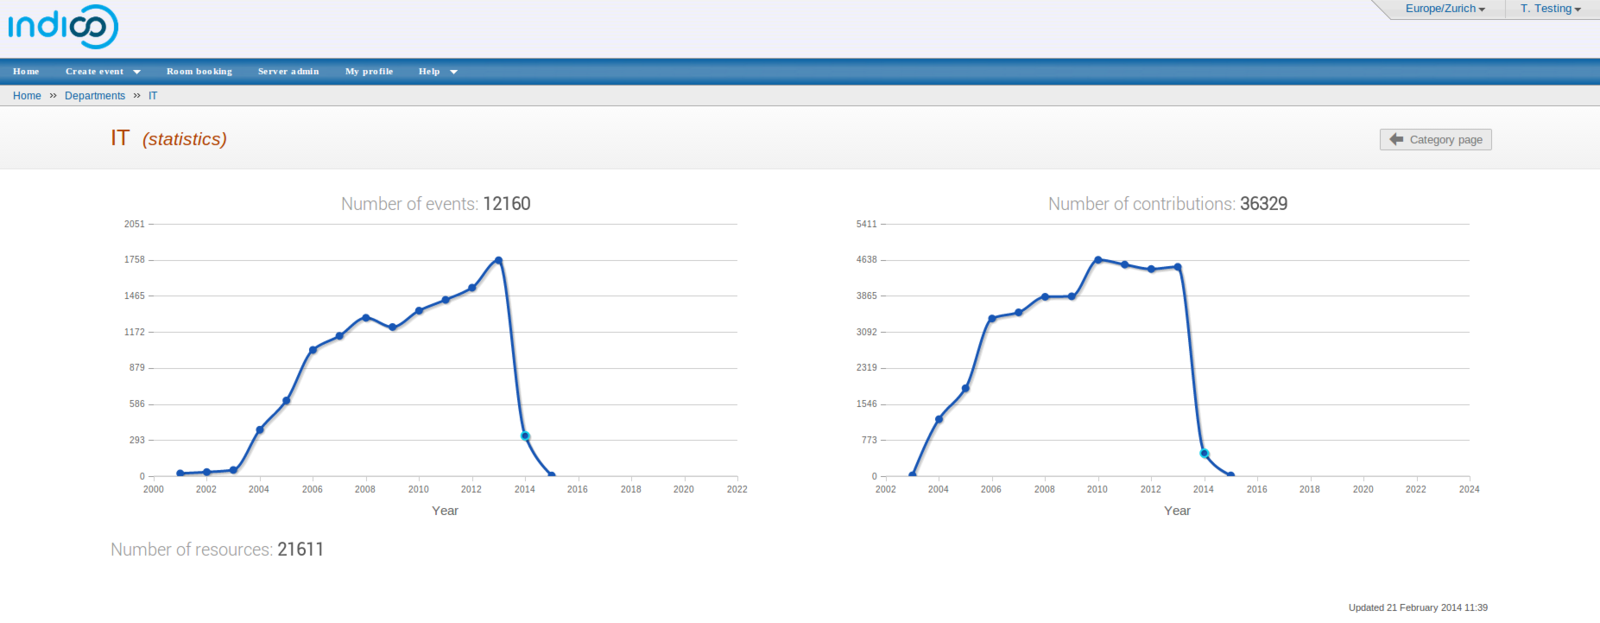
\includegraphics[scale=0.23]{category_statistics.png}
       		\end{center}
       		\caption[Statistiche di una categoria]{Nuova pagina delle statistiche di una categoria in Indico.}
       		\label{fig:category_statistics}
       	\end{figure}

    \section{Installazione su Windows Server} \label{sec:ap;installazione_windows_server}
    
        Uno degli obiettivi del KT Project per Indico includeva l'esplorazione di possibilità per un possibile adattamento di Indico a sistemi Windows Server. Indico infatti è stato progettato per poter essere installato su sistemi Unix e non supporta sistemi Windows. Nell'ottica del Progetto KT, si è tuttavia pensato che molte aziende o organizzazioni potrebbero aver già un server in utilizzo con installato Windows Server. Queste organizzazioni potrebbero essere scoraggiate dall'utilizzare Indico, per il quale dovrebbero installare un secondo server con sistema Unix.
        
        I problemi principali dell'installazione di Indico su Windows Server erano principalmente due: riuscire a installare in ambiente Windows tutte le librerie necessarie a Indico e riuscire a far funzionare \ac{WSGI} col web server messo a disposizione da Windows, \acr{IIS}.
        
        Il problema relativo alle librerie era dovuto al fatto che non tutte le librerie utilizzate da Indico erano state distribuite per Windows. Dopo circa un mese di ricerca, si sono riuscite a trovare su Internet, da fonti ufficiali o meno, tutte le librerie necessarie. Alcune di queste librerie si sono trovate in formato \bash{.exe}, che rappresentava la situazione ottima in quanto le più semplici da installare su Windows. Il resto (la maggior parte) sono state installate da Python egg (\bash{.egg}) o da tarball (\bash{.tar.gz}).
        
        Il problema relativo a \ac{WSGI} stava invece nel riuscire a trovare, installare e configurare un wrapper funzionante per \ac{IIS}. \ac{WSGI} è un'interfaccia che permette la comunicazione tra applicazioni Python e un determinato web server. Per poter far funzionare \ac{WSGI} con un determinato web server, è tuttavia necessario trovare un wrapper adatto, come ad esempio \bash{mod_wsgi} per Apache. Per trovare un wrapper adatto si sono provate diverse soluzioni, come WFastCGI, isapi-wsgi o PyISAPIe (si veda \cite{wiki:wsgi}), ma non sono risultate sufficienti. Si è invece riusciti a far comunicare correttamente \ac{WSGI} con \ac{IIS} tramite un pacchetto sviluppato dalla società HeliconTech e scaricabile al seguente indirizzo: \url{http://www.helicontech.com/zoo/gallery/PythonHostingPackage.html}.
        
        Dopo aver risolto questi due problemi, si era riusciti ad avviare Indico e ad eseguire alcune semplici azioni con esso. Tuttavia Indico presentava ancora seri problemi, come immagini mancanti o alcune librerie non pienamente funzionanti. A questo punto, però, si è deciso di lasciar perdere questo progetto e di dichiarare fallimentare l'installazione di Indico su Windows Server. In fin dei conti, l'installazione su Windows Server rimaneva un progetto minore del KT Project e, al momento, stava già facendo perdere troppo tempo, che sarebbe stato meglio speso su altri progetti più importanti, come l'Instance Tracking.
